% PLOS Computational Biology research article.
\documentclass[11pt,letterpaper]{article}
\usepackage[margin=1in]{geometry}
\usepackage{amsmath,amssymb,amsfonts,bm}
\usepackage{booktabs,tabularx,array}
\usepackage{siunitx}
\usepackage{graphicx}
\usepackage{hyperref,cleveref}
\hypersetup{hidelinks,
  pdftitle={Electrostatic-hydrophobic cooperation in the mesoscale assembly of synapsin and synaptic vesicles},
  pdfauthor={Shokoofeh Akbari, Oleg Shupliakov, Yousef Jamali}}
\usepackage{xurl}
\usepackage{lineno}
\usepackage{setspace}
\usepackage{cite}
\renewcommand{\figurename}{Fig}
\crefname{figure}{Fig}{Figs}
\Crefname{figure}{Fig}{Figs}
\sisetup{detect-all,per-mode=symbol}
\newcommand{\kBT}{k_{\mathrm B}T}
\newcommand{\Syn}{\mathrm{Syn}}
\newcommand{\SV}{\mathrm{SV}}
\newcolumntype{Y}{>{\raggedright\arraybackslash}X}
\bibliographystyle{plos2025}
\begin{document}
\begin{center}
{\LARGE\bfseries Electrostatic--hydrophobic cooperation in the mesoscale
assembly of synapsin and synaptic vesicles\par}
\vspace{0.3em}
{\normalsize Short title: Force control of synapsin--vesicle assemblies\par}
\vspace{0.6em}
{\large Shokoofeh Akbari\textsuperscript{1},
Oleg Shupliakov\textsuperscript{2},
Yousef Jamali\textsuperscript{1,*}\par}
\vspace{0.4em}
\textsuperscript{1}Department of Applied Mathematics, School of Mathematical Sciences,
Tarbiat Modares University, Tehran, Iran\par
\textsuperscript{2}Department of Neuroscience, Karolinska Institutet,
Stockholm, Sweden\par
\textsuperscript{*}Correspondence: y.jamali@modares.ac.ir\par
Yousef Jamali ORCID: \url{https://orcid.org/0000-0002-5709-3821}\par
Shokoofeh Akbari: shokoofe.akbari1997@gmail.com\par
Oleg Shupliakov: oleg.shupliakov@ki.se
\end{center}
\clearpage
\doublespacing
\linenumbers

\begin{abstract}
Synapsin associates with synaptic vesicles, but local association does
not always connect vesicle groups. We used a three-dimensional Brownian
agent model to compare electrostatic and hydrophobic interactions in a
four-condition design at fixed abundance and confinement. Electrostatics
rapidly placed synapsin near almost every vesicle, while larger networks
developed more slowly. With both interactions active, a large connected
assembly formed earlier and synapsin motion was slower. Following all
conditions for 84 ms showed continued growth under either interaction
alone. Their vesicle participation became similar despite different
levels of protein association. The positive early interaction contrast
decreased as these assemblies grew, and the later contrast depended on
which structural measure was used. Contact composition and network
connectivity therefore resolve different stages of synapsin-mediated
organization, from local vesicle coverage to collective assembly.
\end{abstract}

\section*{Author summary}
Synapsin helps organize the vesicles that store neurotransmitters. We
asked whether the interactions that bring synapsin close to vesicles also
connect vesicles into larger groups. In a computer model, electrical
interactions quickly placed synapsin near almost every vesicle. The
vesicles took longer to form large connected groups. Adding hydrophobic
attraction produced a larger assembly earlier and reduced synapsin
motion. When we followed the simulations for longer, both
single-interaction conditions continued to grow. They eventually included
similar fractions of vesicles in their largest groups, although their
protein association remained different. Counting local protein contacts
and measuring connections between vesicles describe different aspects
of assembly. Their relationship also changes as the system develops.

\section{Introduction}
A presynaptic terminal holds synaptic vesicles (SVs) in groups while
allowing them to move and participate in neurotransmission. The protein-rich
SV membrane offers many sites for local interactions \cite{Takamori2006}.
As vesicles and proteins move, these interactions can also link vesicles
into larger assemblies.

Experiments on synapsin have linked molecular interactions to vesicle
organization. Early bilayer experiments identified both electrostatic
association and hydrophobic engagement of the synapsin head domain
\cite{BenfenatiBilayers1989}. Purified-vesicle experiments distinguished
lipid binding from an ionic-strength- and phosphorylation-sensitive
protein-associated contribution \cite{BenfenatiSV1989}. Computational
cage and cytoskeletal cross-linking models then examined how
phosphorylation-dependent binding could redistribute vesicles
\cite{Benfenati1991}. Later, perturbation of an amphipathic lipid-packing
sensor motif linked membrane curvature sensing to synapsin binding and
vesicle clustering \cite{Krabben2011}. Binding and clustering therefore
involve more than one type of interaction.

Reconstitution experiments showed that synapsin assemblies capture
vesicles and disperse following kinase treatment \cite{Milovanovic2018}.
Perturbing the disordered region of synapsin also affects vesicle clusters
in a living lamprey synapse \cite{Pechstein2020}. Single-molecule tracking
linked vesicle sequestration to restricted synapsin motion
\cite{Hoffmann2023}. The mechanism also depends on the synaptic context.
Song and Augustine distinguished synapsin-dependent condensation at
inhibitory synapses from tetramer-mediated cross-linking at excitatory
synapses \cite{Song2023}. Reserve-pool tracking also implicated Synapsin 2a
tetramerization in vesicle organization \cite{Longfield2024}. These
findings motivate separate measures of protein association, vesicle
connectivity and particle motion.

Microscopy and a binding-particle model related assembly size and
morphology to the synapsin-to-lipid ratio and vesicle adhesion
\cite{Alfken2024}. X-ray scattering and cluster simulations resolved
noncompact SV--synapsin assemblies with close intervesicle contacts
\cite{Neuhaus2024}. More recent X-ray microrheology of synapsin assemblies
with colloid-supported lipid bilayers found concentration-dependent motion
and relaxation \cite{Czajka2026}. Together, these studies measure assembly
structure and dynamics at different scales.

Simulation approaches span several resolutions. Atomistic synapsin
simulations coupled to experiments revealed an ATP-dependent
conformational route to vesicle binding and oligomerization
\cite{Orlando2014}. Residue-level models resolve charge and hydropathy
along protein chains \cite{Dignon2018}, while coarse-grained simulations
of repetitive peptides show that the balance of electrostatic repulsion
and hydrophobic attraction depends on sequence and solution conditions
\cite{Yang2024}. At the particle level, the synapsin--vesicle model of
Alfken et al.\ addresses binding redistribution and finite assembly size
\cite{Alfken2024}. An agent model can represent thousands of moving
proteins and vesicles while retaining their identities and pair interactions.
We use this resolution to test how electrostatic and hydrophobic interactions
change collective organization at fixed abundance and confinement. Random-graph and
continuum-percolation studies show how connectivity can change
nonlinearly with the number and organization of edges
\cite{NewmanStrogatzWatts2001,DallChristensen2002}. This framework lets us
ask how local synapsin association relates to the wider vesicle population.

We vary electrostatic and hydrophobic interactions independently in a
three-dimensional Brownian agent model. Particle abundance, confinement
and dispersion attraction remain fixed. Species-resolved contact networks
measure protein association and vesicle connectivity. Saved trajectories
also allow a mobility comparison with published tracking data. The
comparison shows how the two interactions shape local association and
collective vesicle organization.

\section{Results}
The four conditions differ in the electrostatic (E) and hydrophobic (H)
interactions. Particle population and confinement are the same. Each
condition has three independent simulation runs, followed for 84 ms.
Structural comparisons use the final 180 saved frames, from 58.94 to
84 ms. We also retain the earlier 28-ms comparison to examine how the
response develops with time.

\subsection{Combined interactions produce an earlier and larger connected assembly}
With neither E nor H active, the late mean all-agent largest-component
fraction was 0.0368. It reached 0.3440 with H alone, 0.5025 with E alone
and 0.9200 with both interactions
(\cref{tab:force-means,fig:force-endpoints}). The combined-interaction
condition had the largest component in every seed at both observation
horizons.

\begin{table}[htbp]\centering\small
\caption{Structural outcomes over 58.94--84 ms at the primary 2-nm association shell.}
\label{tab:force-means}
\begin{tabular}{@{}lccc@{}}\toprule
Condition & All-agent largest component & Non-isolated Syn & SVs in largest component \\
\midrule
E0H0 & 0.0368 (0.0150) & 0.3172 (0.0035) & 0.1143 (0.0492) \\
E0H1 & 0.3440 (0.0667) & 0.5678 (0.0221) & 0.5229 (0.0783) \\
E1H0 & 0.5025 (0.0847) & 0.7639 (0.0142) & 0.5323 (0.0728) \\
E1H1 & 0.9200 (0.0064) & 0.9516 (0.0023) & 0.8909 (0.0204) \\
\bottomrule\end{tabular}
\par\smallskip\raggedright
Entries are means across three independent seeds with between-seed SD in
parentheses. E and H denote the electrostatic and hydrophobic kernels;
van der Waals attraction is present in every row.
\end{table}

\begin{figure}[tbp]\centering
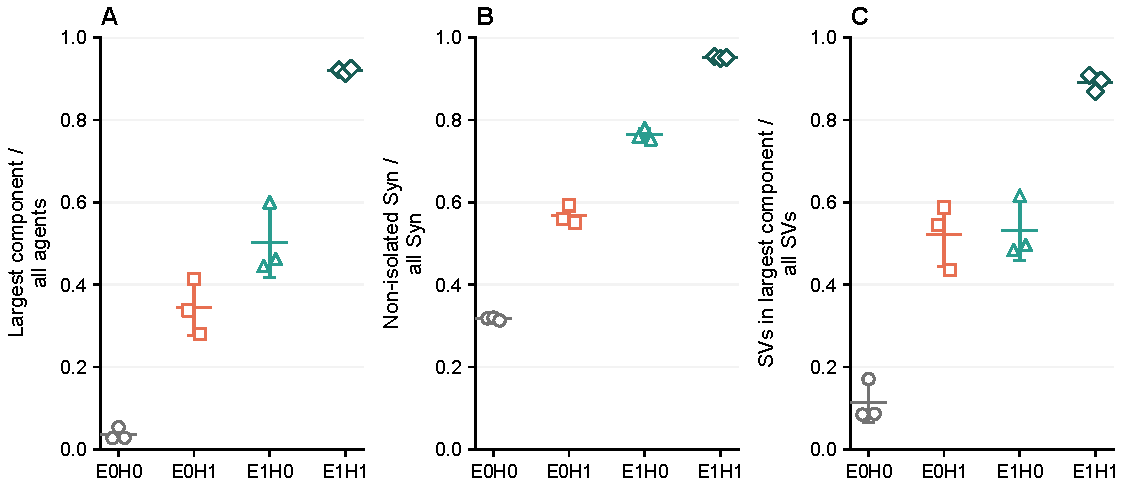
\includegraphics[width=\linewidth]{figures/force_factorial_endpoints.pdf}
\caption{Late-window responses to the electrostatic (E) and hydrophobic
(H) interactions at the 2-nm graph shell, averaged over 58.94--84 ms.
Open symbols show individual runs; horizontal marks and bars show the
mean and one between-seed SD ($n=3$ per condition). Non-isolated synapsin
includes Syn--Syn and Syn--SV components. Van der Waals attraction is
active throughout.}
\label{fig:force-endpoints}
\end{figure}

The time courses show a clear difference in how quickly the assemblies
developed (\cref{fig:force-time}A). At 28 ms, the mean all-agent
largest-component fractions were 0.020, 0.090, 0.099 and 0.610 for
E0H0, E0H1, E1H0 and E1H1. At 84 ms, they were 0.034, 0.409, 0.595 and
0.926. The E1H1 growth slowed at later times: its mean fitted slope
decreased from 0.0148 per ms over 14--28 ms to 0.00038 per ms over
70--84 ms (\cref{fig:force-time}C). The single-interaction conditions
continued to grow during the extended observation.

For each seed, we compared joint activation with the sum of the separate
E and H effects, using E0H0 as the common background:
\begin{equation}
 \Delta_{EH}=(Y_{11}-Y_{10})-(Y_{01}-Y_{00}).
 \label{eq:interaction-effect}
\end{equation}
For the all-agent largest-component fraction, the early late-window
contrast over 19.74--28 ms was 0.3723 and positive in all three seeds.
Over 58.94--84 ms, its mean decreased to 0.1103, with seed values
0.1660, $-0.0463$ and 0.2112. Growth under E or H alone reduced the
initial separation from their additive reference.

\begin{figure}[tbp]\centering
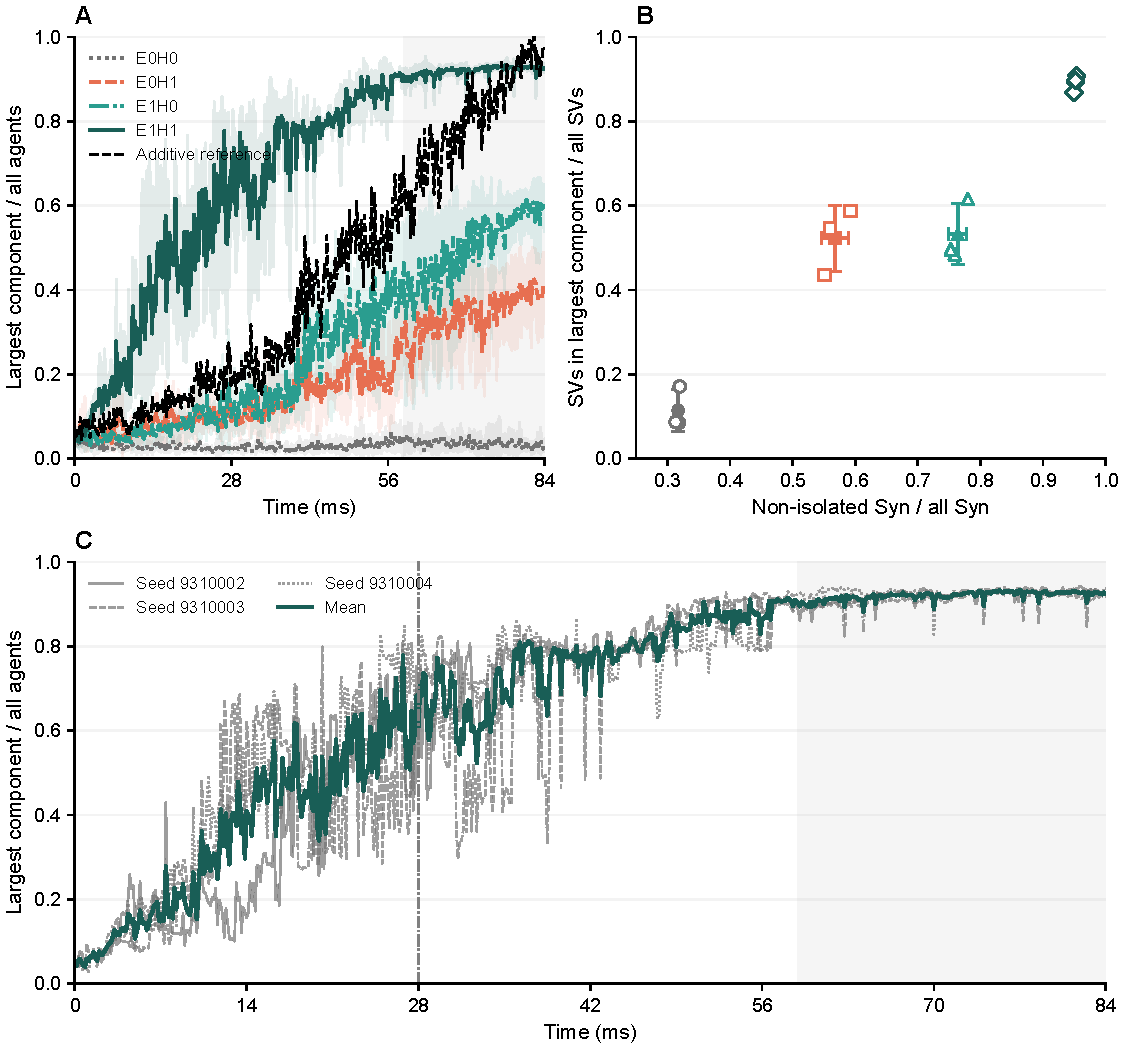
\includegraphics[width=\linewidth]{figures/force_factorial_timecourse.pdf}
\caption{Network growth and vesicle participation at the 2-nm graph shell.
(A) All-agent largest-component fraction for all four conditions through
84 ms. Lines show condition means, bands show one between-seed SD,
and the dashed line is the additive reference
$\overline L_{10}(t)+\overline L_{01}(t)-\overline L_{00}(t)$.
Shading marks the final 180 frames. (B) Late-window non-isolated synapsin
versus SV participation in the largest component. Open symbols show runs;
filled symbols and bars show means and one SD. (C) The three E1H1
trajectories and their mean. The vertical line marks 28 ms; shading
marks 58.94--84 ms.}
\label{fig:force-time}
\end{figure}

\subsection{Protein association and vesicle participation follow different time courses}
Electrostatics produced the larger increase in the non-isolated synapsin
fraction $Q_{\Syn}$. At 84 ms, its late-window mean was 0.7639 with E
alone and 0.5678 with H alone (\cref{tab:force-means}). The corresponding
SV fractions in the largest component, $L_{\SV}$, were similar:
0.5323 and 0.5229. The two conditions therefore had different protein
participation despite comparable collective vesicle participation.

This relationship developed over time. In the earlier 19.74--28-ms
window, E alone gave more non-isolated synapsin than H alone
(0.6989 versus 0.5157), but fewer SVs in the largest component
(0.1273 versus 0.1839). That ordering of vesicle participation held
in every seed at 28 ms. The longer observation shows that it describes
an early stage of assembly.

With both interactions active, the 84-ms late-window means reached
0.9516 for $Q_{\Syn}$ and 0.8909 for $L_{\SV}$.
Their E-by-H contrasts were $-0.0628$ and $-0.0500$, respectively.
For $L_{\SV}$, the seed contrasts were $-0.0369$, $-0.1642$ and 0.0509,
compared with three positive values and a mean of 0.3811 at 28 ms.
The conditional differences are given in \cref{tab:force-contrasts}.
The interaction contrast thus depends on the structural observable
and the observation period.

\begin{table}[htbp]\centering\small
\caption{Paired seed-block contrasts over 58.94--84 ms at the 2-nm shell.}
\label{tab:force-contrasts}
\begin{tabular}{@{}llc@{}}\toprule
Outcome & Conditional contrast & Mean difference (SD) \\
\midrule
All-agent largest component & H effect at E0 & 0.3072 (0.0538) \\
 & H effect at E1 & 0.4175 (0.0906) \\
 & E effect at H0 & 0.4656 (0.0698) \\
 & E effect at H1 & 0.5760 (0.0730) \\
\addlinespace
Non-isolated Syn & H effect at E0 & 0.2506 (0.0194) \\
 & H effect at E1 & 0.1877 (0.0159) \\
 & E effect at H0 & 0.4466 (0.0115) \\
 & E effect at H1 & 0.3838 (0.0238) \\
\addlinespace
SVs in largest component & H effect at E0 & 0.4086 (0.0562) \\
 & H effect at E1 & 0.3586 (0.0929) \\
 & E effect at H0 & 0.4180 (0.0239) \\
 & E effect at H1 & 0.3680 (0.0900) \\
\bottomrule\end{tabular}
\par\smallskip\raggedright
Values are mean differences in fractions, with the SD of the three
paired seed differences in parentheses. ``H effect'' means H1--H0
at fixed E; ``E effect'' means E1--E0 at fixed H.
\end{table}

\subsection{Local vesicle coverage and connections between groups}
We separated Syn--Syn, Syn--SV and SV--SV contacts in the saved frames.
At the 2-nm shell, the 84-ms late-window fraction of synapsin next to
at least one SV was 0.1906 in E0H0, 0.4647 in E0H1, 0.7508 in E1H0
and 0.9499 in E1H1 (\cref{fig:interface-diagnostics}).

Electrostatics alone already gave broad SV coverage at 28 ms: 99.72\%
of SVs had a synapsin neighbor, although only 12.73\% belonged to the
largest component. At 84 ms, the corresponding late-window values were
99.14\% and 53.23\%. Extensive local coverage therefore preceded
collective vesicle connectivity. In E1H1, 98.08\% of SVs had a synapsin
neighbor and 89.09\% belonged to the largest component in the later
window.

The late-window fraction of synapsin next to at least two SVs was
0.1454 with H alone, 0.2097 with E alone and 0.6688 with both
interactions (\cref{fig:interface-diagnostics}B). Mean Syn--SV edge
counts per snapshot were 1,140.6, 1,735.7 and 2,985.4, respectively.
The joint condition also had more Syn--Syn edges, with a mean of
1,372.8, compared with 469.2 under H alone and 314.5 under E alone.
Its many multivesicle neighbors provide geometric connections between
vesicles within the association graph.

The single-interaction conditions differed in contact composition.
E1H0 had more total edges than E0H1 (2,082.0 versus 1,793.9 per
snapshot), but fewer Syn--Syn and SV--SV edges. Their similar
$L_{\SV}$ values at 84 ms therefore arose from different local contact
networks. Their all-agent largest-component fractions remained more
distinct because that measure also counts synapsin particles.

\begin{figure}[tbp]\centering
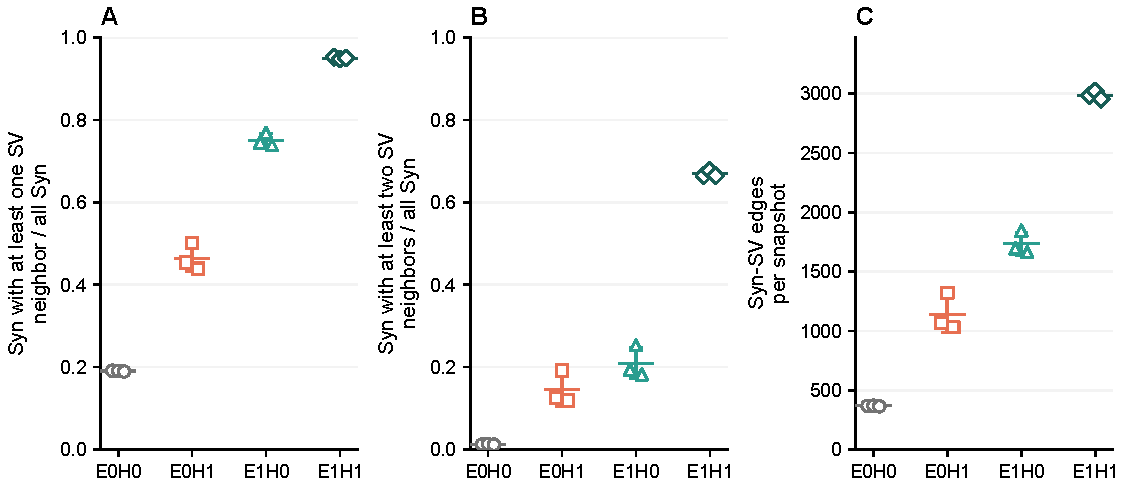
\includegraphics[width=\linewidth]{figures/force_interface_diagnostics.pdf}
\caption{Species-resolved contacts over 58.94--84 ms at the 2-nm graph shell.
(A) Fraction of Syn agents adjacent to at least one SV.
(B) Fraction adjacent to at least two distinct SVs.
(C) Number of Syn--SV edges per snapshot. Open symbols show individual
late-window run means; marks and bars show the mean and one between-seed
SD ($n=3$ per condition). Contact uses outer radii, including the SV
corona.}
\label{fig:interface-diagnostics}
\end{figure}

\subsection{The joint condition retains the largest assembly across observation shells}
Across 0, 2, 4 and 6 nm surface-gap shells, E1H1 retained the largest
mean all-agent component and largest-component SV fraction at 84 ms.
Its all-agent fraction ranged from 0.8872 to 0.9382, compared with
0.0185--0.1433 for E0H0. The ordering was consistent across these
graph thresholds applied to the same trajectories.

\subsection{Stronger assembly accompanies slower short-lag motion}
We estimated synapsin mobility from saved positions projected onto the
$xy$ plane. Apparent diffusion coefficients came from fits to each
agent's time-averaged mean-squared displacement (MSD) over lags of
2.10--3.92 ms. For the full 84-ms trajectories, across-seed means of
the agent-mean apparent coefficient were 0.1403, 0.1308, 0.1108 and
$0.0626\,\si{\micro\metre\squared\per\second}$ for E0H0, E0H1, E1H0
and E1H1, respectively (\cref{fig:mobility-comparison}). Mobility
was about 55\% lower in E1H1 than in E0H0.

The released Hoffmann et al.\ source data provide an experimental scale
reference. They report a mean short-time synapsin coefficient of
$0.0189\,\si{\micro\metre\squared\per\second}$ with SVs, versus
$0.0253\,\si{\micro\metre\squared\per\second}$ without SVs
\cite{Hoffmann2023}. The E1H1 full-trajectory mean is about 3.3 times
the experimental with-SV mean. Restricting the simulation analysis to
58.94--84 ms gives an E1H1 mean of
$0.0548\,\si{\micro\metre\squared\per\second}$. Both the experimental
and simulated comparisons show lower synapsin mobility in the more
assembled setting. S1 Text gives the per-run estimates and their
window sensitivity.

\begin{figure}[tbp]\centering
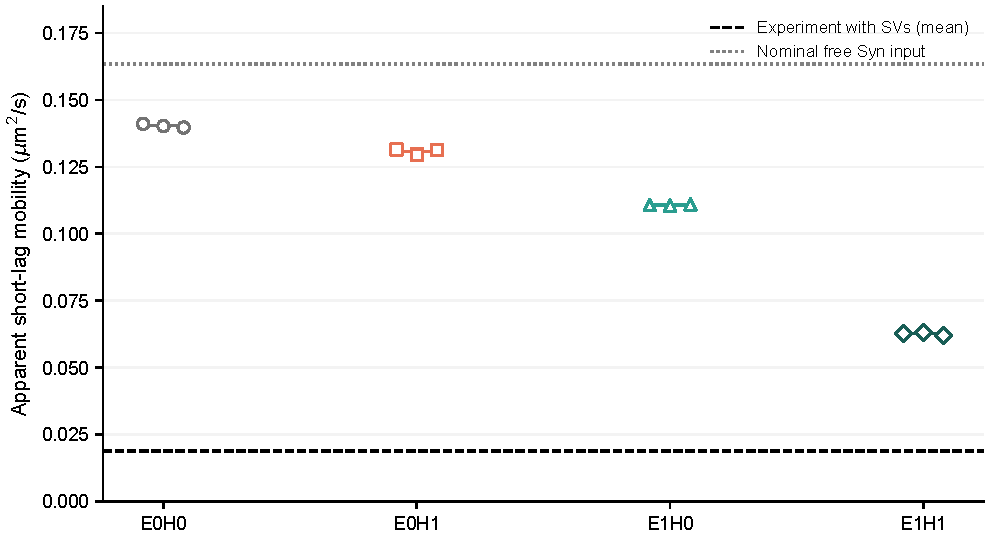
\includegraphics[width=0.88\linewidth]{figures/force_mobility_external_comparison.pdf}
\caption{Short-lag synapsin mobility over the full 84-ms trajectories and
the experimental reference. Symbols show run means over synapsin agents;
marks and bars show the between-seed mean and one SD. The apparent
coefficient is one quarter of the free-intercept slope of projected
time-averaged MSD over 2.10--3.92 ms. The dashed line is the Hoffmann
et al.\ with-SV mean from released Fig.~2h source data
\cite{Hoffmann2023}. The dotted line shows the nominal unconfined
synapsin diffusion coefficient.}
\label{fig:mobility-comparison}
\end{figure}

\section{Discussion}
\subsection{Local association and collective organization develop on different time scales}
The extended trajectories separate early vesicle coverage from the
subsequent growth of connected assemblies. Electrostatics alone placed
synapsin near almost every vesicle by 28 ms. At that stage, most
vesicles still belonged to separate groups. Their participation in the
largest component increased over the next 56 ms while local coverage
remained high. With both interactions active, a large connected
assembly formed earlier and its growth slowed towards 84 ms.

The pair forces help explain the contact networks (\cref{tab:pair-scope}).
Electrostatics attracts Syn--SV pairs and repels like-species pairs.
Hydrophobic attraction acts on Syn--Syn and Syn--SV pairs. E1H0
favored Syn--SV contacts, while E0H1 had more Syn--Syn and SV--SV
contacts. At 84 ms, the two conditions had similar fractions of
vesicles in the largest component despite different levels of
synapsin participation. Joint activation produced many more synapsin
particles close to several vesicles, which can connect vesicles in
the association graph.

\begin{table}[htbp]\centering\small
\caption{Pair-level action of the two interaction terms at positive outer-surface gap.}
\label{tab:pair-scope}
\begin{tabular}{@{}lll@{}}\toprule
Pair class & Electrostatic interaction when E1 & Hydrophobic interaction when H1 \\
\midrule
Syn--Syn & Repulsive & Attractive \\
Syn--SV  & Attractive & Attractive \\
SV--SV   & Repulsive & Zero amplitude \\
\bottomrule\end{tabular}
\par\smallskip\raggedright
Signs describe radial forces for the assigned effective surface
potentials. Dispersion attraction acts in all three pair classes and
remains enabled in every condition.
\end{table}

Connectivity changes nonlinearly with the number and placement of
edges, as in random graphs and continuum percolation
\cite{NewmanStrogatzWatts2001,DallChristensen2002}. Here, the large
positive interaction contrast at 28 ms decreased as the
single-interaction assemblies grew. At 84 ms, the all-agent contrast
was positive on average with mixed seed signs, while the mean
vesicle-participation contrast was slightly negative. The joint
condition still had the largest assembly. These results connect the
early cooperative response to the timing of network growth and to the
structural measure used. Experiments that follow local vesicle
coverage and group connectivity over time could distinguish these
stages during perturbations of protein--membrane and protein--protein
interactions.

\subsection{Relation to molecular and particle-level models}
The particle model of Alfken et al.\ links redistribution of vesicle-bound
synapsin to adhesion and finite assembly size \cite{Alfken2024}. Their
two-dimensional periodic Langevin model follows proteins on vesicle
surfaces. Our model follows freely moving effective synapsin particles
inside a three-dimensional compartment and separates electrostatic from
hydrophobic interactions. The two models address different routes from
local interaction to vesicle assembly.

Residue-level simulations describe charge and hydropathy along protein
chains \cite{Dignon2018}. In repetitive peptides, hydrophobic attraction
competes with same-sign electrostatic repulsion \cite{Yang2024}. Our
two-species model represents this competition for Syn--Syn pairs and
includes attraction between oppositely charged Syn--SV pairs. The latter
favors local protein association, while larger vesicle assemblies also
depend on how the contacts connect separate groups.

Atomistic simulations and experiments connect an ATP-dependent synapsin
conformational transition to vesicle binding and oligomerization
\cite{Orlando2014}. At the mesoscale, our contact-network analysis shows
how the balance of effective interactions changes the organization of
many vesicles.

\subsection{Experimental context and biological implications}
Reconstitution and neuronal experiments establish synapsin as a regulator
of vesicle organization \cite{Milovanovic2018,Pechstein2020}. Scattering
measurements show noncompact synapsin--vesicle clusters \cite{Neuhaus2024}.
Their structure makes connected-component measures relevant alongside
cluster size. Studies of synaptophysin tails also support electrostatic
interactions in protein--vesicle assembly \cite{Park2021,Kim2021}.

Joint activation reduced short-lag synapsin mobility by about 55\%
relative to E0H0. Hoffmann et al.\ likewise observed restricted synapsin
motion in the presence of vesicles \cite{Hoffmann2023}. The simulated
apparent diffusion coefficient was about 3.3 times their with-SV mean.
A quantitative mobility match would require further calibration.

The distinction between coverage and connectivity may also help interpret
synapsin dysfunction. Human
\textit{SYN1} loss-of-function variants associated with autism and epilepsy
impair vesicle-pool size and trafficking \cite{Fassio2011}. Oxidation and
persulfidation have been linked to different changes in synapsin
condensation and neurotransmission \cite{Vignane2026}. Together, these
studies motivate experiments that measure local vesicle association and
network connectivity.

\subsection{Scope and limitations}
All four conditions were followed for 84 ms. Growth of the E1H1
largest component slowed markedly, while the single-interaction
conditions were still developing. The reported contrasts describe
assembly over a common observation period. Their change between 28
and 84 ms makes observation time part of the comparison. Three seed
blocks give limited precision for the later interaction contrasts.
We studied one concentration and compartment volume; other
concentrations may change the response near a connectivity threshold
or saturation.

The agents are spheres with effective surface interactions in a closed
compartment. Switching E or H changes several pair classes at once.
Pair-specific perturbations would resolve their separate contributions.
Graph edges describe proximity. A synapsin near several vesicles is
counted as a multivesicle contact; molecular binding is unresolved.
The model omits explicit valency, phosphorylation, membrane deformation,
active vesicle cycling and hydrodynamic coupling. Numerical checks
establish geometric admissibility; convergence of the reported observables
at smaller integration steps remains to be assessed. Connectivity and
short-lag motion characterize assembly here. A claim of liquid--liquid
phase separation would also need evidence for phase coexistence,
exchange and system-size behavior.

The mobility reference has different sampling: Hoffmann et al.\ selected
condensate-core tracks, while our estimate includes every synapsin agent
and uses a different saved cadence without localization noise. The
3.3-fold difference in apparent mobility is a scale comparison, pending
calibration against matched tracking conditions. The interaction
switches likewise do not represent specific disease variants or
biochemical modifications.

\subsection*{Conclusion}
Electrostatic and hydrophobic interactions shape both the timing and
the structure of synapsin--vesicle assembly. Electrostatics rapidly
gave broad local vesicle coverage. Collective connectivity developed
more slowly under either interaction alone, while their combination
produced a larger assembly earlier and lower short-lag synapsin
mobility. Following all conditions to 84 ms resolved how the early
interaction contrast changed as the separate assemblies grew.
Local contact abundance, particle composition and vesicle
connectivity describe complementary aspects of this process.

\section{Methods}
\subsection{Simulation design and numerical settings}
The four force conditions each have three independent seed blocks
(9310002--9310004), giving 12 trajectories. Every run contains 200 SVs
and 1,807 synapsin agents in a closed $0.1\,\mu$m$^3$ compartment. Each
trajectory comprises 120,000 integration steps and 600 saved frames.
The original 28-ms trajectories were continued from checkpoints after
inspection showed continuing growth. Physical parameters and the random
number generator state were retained; duplicate join frames were counted once.
The numerical settings are common to all conditions. S1 Text gives the
per-run numerical diagnostics.

\subsection{Compartment, size distributions, and population}
We represent SVs and synapsin as spherical agents in three dimensions,
following the scale of synapsin--vesicle reconstitution and neuronal
imaging \cite{Milovanovic2018,Hoffmann2023}. The closed spherical
compartment has volume
\(V=\SI{0.10}{\micro\metre\cubed}\), corresponding to radius
\begin{equation}
 R_{\mathrm b}=\left(\frac{3V}{4\pi}\right)^{1/3}
 =\SI{287.94}{\nano\metre}.
 \label{eq:box-radius}
\end{equation}
The scale is informed by three-dimensional hippocampal bouton reconstructions
\cite{Schikorski1997}. An SV has membrane-core radius \(b_i\), corona thickness
\(s_i=\SI{4.8}{\nano\metre}\), and outer radius \(a_i=b_i+s_i\).
Synapsin has \(b_i=a_i=\SI{3.972}{\nano\metre}\) and \(s_i=0\).
The protein corona is interpenetrable \cite{Neuhaus2024}; the synapsin
radius sets the effective particle size.

SV core radii are independently rejection-sampled from a normal distribution
with location \(\mu_R=\SI{20.45}{\nano\metre}\) and input SD
\(\sigma_R=\SI{2.5}{\nano\metre}\), restricted to
\(15\leq b_i\leq30\,\si{\nano\metre}\). The mean and SD inputs follow the
excitatory-SV diameter measurements of Tao et al.\ \cite{Tao2018}; the bounds
are informed by cryo-electron microscopy (cryo-EM) and small-angle
X-ray scattering (SAXS) size measurements \cite{Castorph2010}. These
values specify the distribution before truncation. Synapsin counts
are obtained from
\begin{equation}
 N_{\Syn}=\left\lfloor N_{\mathrm A}C_{\Syn}V+\frac12\right\rfloor.
 \label{eq:count}
\end{equation}
Here \(N_{\mathrm A}\) is Avogadro's constant, with \(C_{\Syn}\) in
\(\si{\mole\per\metre\cubed}\) and \(V\) in \(\si{\metre\cubed}\);
\(\lfloor x+1/2\rfloor\) rounds a nonnegative value to the nearest integer.
The chosen \(30\,\si{\micro\mole\per\litre}\) concentration gives
\(N_{\Syn}=1807\).
There are 200 SVs at the canonical volume. Initial centers are sampled
uniformly within active cells and restricted to the particle-accessible
sphere. Before the physical trajectory, an overlap-relaxation stage
reduces initial core intersections. Its stopping criterion is an overlap
below \SI{0.05}{\nano\metre} for three checks, or no overlapping pairs;
the stage has a 200-iteration ceiling.

\subsection{Linked cells and boundary treatment}
The supremum outer SV diameter is \(d_{\max}=2(30+4.8)
=\SI{69.6}{\nano\metre}\). For each bounding-box dimension \(L_d\), the grid uses
\begin{equation}
 n_d=\max\{1,\lfloor L_d/d_{\max}\rfloor\},\qquad h_d=L_d/n_d.
 \label{eq:cells}
\end{equation}
The canonical sphere has eight cells per bounding-box axis, with
\(h_d=\SI{71.9853}{\nano\metre}\). Cells are assigned by particle center.
The force calculation searches the home cell and two neighboring cell
layers. Every candidate pair enters the force calculation; no further
radial cutoff is imposed.

The largest center distance at a 6-nm outer-surface gap is
\(d_{\max}+6=\SI{75.6}{\nano\metre}\), within the two-layer search
distance of \SI{143.9706}{\nano\metre}.
A particle center is confined to radius \(R_{\mathrm b}-a_i\) from the
compartment center. Out-of-domain proposals are mapped inward by radial
folding; the same boundary map is applied after overlap corrections.
The resulting boundary approximates a closed reflecting wall.

\subsection{Pair interactions}
Let \(r_{ij}=\lVert\bm x_i-\bm x_j\rVert\),
\(\bm n_{ij}=(\bm x_i-\bm x_j)/r_{ij}\), and
\(g_{ij}=r_{ij}-a_i-a_j\). A positive radial force is repulsive.
The production force definition is
\begin{equation}
 \bm F_i=\sum_{j\in\mathcal N_i}
 \mathbf 1\{g_{ij}\geq0\}
 \left(E f_{ij}^{E}+H f_{ij}^{H}+f_{ij}^{W}\right)\bm n_{ij}.
 \label{eq:total-force}
\end{equation}
Here \(\mathcal N_i\) is the linked-cell candidate set and
$E,H\in\{0,1\}$ switch the electrostatic and hydrophobic terms.
Van der Waals attraction remains active in every condition. At negative
outer gap, the surface-force terms vanish and geometric correction
controls core overlap.

The electrostatic kernel is a reduced-potential, screened sphere interaction:
\begin{align}
 f_{ij}^{E}
 &=\kBT\frac{a_i a_j}{\ell_{\mathrm B}}\,
   \varphi_i\varphi_j e^{-\kappa g_{ij}}
   \left(\frac{1}{r_{ij}^{2}}+\frac{\kappa}{r_{ij}}\right),
 \label{eq:electrostatic}\\
 \varphi_i&=\frac{e\psi_i}{\kBT},\quad
 \ell_{\mathrm B}=\frac{e^2}{4\pi\epsilon_0\epsilon_r\kBT},\quad
 \kappa^2=\frac{2e^2N_{\mathrm A}(1000I)}
                 {\epsilon_0\epsilon_r\kBT}.
\end{align}
The last expression uses SI quantities and \(I\) in
\(\si{\mole\per\litre}\); lengths are then converted to nanometers.
At \(T=\SI{310.15}{\kelvin}\), \(\epsilon_r=74.2\), and
\(I=\SI{0.15}{\mole\per\litre}\), \(\kappa^{-1}=\SI[group-digits=false]{0.77886}{\nano\metre}\).
SV and synapsin effective potentials are respectively \(-22.5\) and
\(+16\,\si{\milli\volt}\). Negative isolated-SV zeta potentials motivate
the former \cite{Shin2010}; the latter represents an effective positive
protein charge scale. The kernel approximates screened electrostatics in
a linearized-Poisson--Boltzmann/Yukawa form.

Hydrophobic attraction is
\begin{equation}
 f_{ij}^{H}=-\frac{\epsilon_{ij}\kBT}{\lambda_H}
                  e^{-g_{ij}/\lambda_H},
 \qquad \lambda_H=\SI{0.5}{\nano\metre}.
 \label{eq:hydrophobic}
\end{equation}
This follows from \(U_{ij}^{H}=-\epsilon_{ij}\kBT
e^{-g_{ij}/\lambda_H}\) outside contact. An exponential kernel has a
surface-force precedent \cite{Israelachvili1982}; its length and pair
amplitudes specify the effective short-range attraction. The SV--SV
hydrophobic amplitude is zero.

For the fixed dispersion background, the membrane/core radii are used:
\begin{equation}
 f_{ij}^{W}=-\frac{A\,b_i b_j}{6(b_i+b_j)\widehat h_{ij}^{\,2}},
 \qquad
 \widehat h_{ij}=\max\{r_{ij}-b_i-b_j,h_0\},
 \label{eq:vdw}
\end{equation}
where \(A=\SI{5e-21}{\joule}\) and \(h_0=\SI{0.3}{\nano\metre}\).
This non-retarded Hamaker--Derjaguin approximation is informed by dispersion
theory \cite{Hamaker1937}; it uses a common effective aqueous background
constant. The dispersion surfaces are defined by core radii, with lower-gap
regularization to bound the attraction near contact.

\subsection{Mobility and discrete stochastic dynamics}
Independent-particle Stokes drag gives
\begin{equation}
 \gamma_i=6\pi\eta_{\mathrm{eff}}a_i,\qquad
 M_i=\gamma_i^{-1},\qquad D_i=\kBT M_i .
 \label{eq:mobility}
\end{equation}
Brownian particle updates use diagonal mobility
\cite{Ermak1978}.
The effective friction input is
\(\eta_{\mathrm{eff}}=\SI{0.35}{\pascal\second}\), selected with reference to
published mobility scales \cite{Hoffmann2023,Rothman2016}.
The nominal unconfined diffusion coefficients are
\(0.1634\,\si{\micro\metre\squared\per\second}\) for synapsin and
\(0.02571\,\si{\micro\metre\squared\per\second}\) for an SV with
\(a_i=\SI{25.25}{\nano\metre}\).

At each Euler--Maruyama step,
\begin{align}
 \bm d_i^n&=M_i\bm F_i(\bm x^n)\Delta t,\qquad
 c_i^n=\min\left\{1,\frac{a_i/4}{\lVert\bm d_i^n\rVert}\right\},\\
 \bm y_i&=\mathcal B_i\left(
       \bm x_i^n+c_i^n\bm d_i^n+
       \sqrt{2D_i\Delta t}\,\bm\xi_i^n\right),\qquad
 \bm\xi_i^n\sim N(\bm0,\bm I_3).
 \label{eq:proposal}
\end{align}
For zero drift, \(c_i^n=1\). The limiter acts on deterministic
displacement, while the Brownian increment remains Gaussian.
\(\mathcal B_i\) is the boundary map.
The next state is the result of mobility-weighted iterative overlap
correction applied to \(\bm y\). Pair admissibility is
\begin{equation}
 r_{ij}\geq b_i+b_j-\delta_0,\qquad
 \delta_0=\SI{0.5}{\nano\metre}.
 \label{eq:admissible}
\end{equation}
Thus permitted outer overlaps are \SI{0.5}{\nano\metre} for Syn--Syn,
\SI{5.3}{\nano\metre} for Syn--SV, and \SI{10.1}{\nano\metre} for SV--SV.
Corrections are accumulated simultaneously, averaged over each particle's
violating contacts, reflected at the wall, and repeated with updated cells.
The residual tolerance is \SI{0.005}{\nano\metre}, with early stopping and a
128-iteration safety ceiling.

The fixed integration step is \(\Delta t=\SI{0.0007}{\milli\second}\).
Each trajectory has 120,000 physical moves over \SI{84}{\milli\second};
snapshots are scheduled every 200 steps, or \SI{0.14}{\milli\second}.
Forces are evaluated at the stored state before movement, aligning saved
forces and positions.

\subsection{Structural graphs and observables}
A nonperiodic undirected graph is constructed independently at each stored
frame using \(A_{ij}^{(\ell)}=\mathbf1\{g_{ij}\leq\ell\}\), \(i\ne j\).
The primary outer-surface shell is \(\ell=\SI{2}{\nano\metre}\), with
\(0,2,4,6\,\si{\nano\metre}\) sensitivity shells. Edges represent geometric
association. Let \(\mathcal C_f\) be the
connected components at frame \(f\), \(n_c=|c|\), and \(c_f^*\) the component
with the largest total agent count. The species-resolved structural
observables are
\begin{align}
 L_{\SV,f}&=\frac{|c_f^*\cap\SV|}{N_{\SV}},\\
 Q_{\Syn,f}&=\frac{\sum_{c\in\mathcal C_f:n_c\geq2}|c\cap\Syn|}{N_{\Syn}} .
 \label{eq:endpoints}
\end{align}
Thus $L_{\SV,f}$ counts vesicles in the component selected by total agent
count, and $Q_{\Syn,f}$ counts synapsin in any component containing at
least two agents, including Syn--Syn groups. The primary structural
observable is the all-agent largest
component fraction
\begin{equation}
 L_{\mathrm{all},f}=\frac{|c_f^*|}{N_{\SV}+N_{\Syn}},
 \label{eq:all-largest}
\end{equation}
while $Q_{\Syn,f}$ and $L_{\SV,f}$ describe local protein participation
and collective vesicle participation, respectively.

Each outcome is averaged over the last
\(m=\max\{1,\lceil0.30F\rceil\}\) of the \(F\) stored frames:
\begin{equation}
 Y_{o,s}=\frac1m\sum_{f=F-m+1}^{F} O_{o,s,f}.
 \label{eq:late-summary}
\end{equation}
Here \(o\) indexes the observable, \(s\) the seed and \(f\) the saved
frame; the force-condition index is suppressed. Each run is summarized
before values are compared across seeds. For these trajectories, the
84-ms late window covers frames 421--600 (58.94--84 ms).
The earlier comparison uses the same 30\% rule on the first 200 frames,
giving frames 141--200 (19.74--28 ms).


\subsection{Force-factorial design}
The factorial design fixes ionic strength at
$I=0.15\,\si{\mole\per\litre}$ and nominal synapsin concentration at
$30\,\si{\micro\mole\per\litre}$. It includes all four combinations
of the binary interaction switches,
$E,H\in\{0,1\}$.
H1 uses the reference amplitudes $\epsilon_{\Syn\Syn}=1.50$ and
$\epsilon_{\Syn\SV}=1.00$, corresponding to well depths of $1.50\kBT$
and $1.00\kBT$, respectively, with
$\epsilon_{\SV\SV}=0$; H0 sets all hydrophobic amplitudes to zero.
E1 uses the electrostatic kernel of \cref{eq:electrostatic} and E0 sets
that kernel to zero. In every condition, the same van der Waals law and its
parameters remain active.

Three seed blocks, 9310002--9310004, were completed in all four conditions.
An earlier four-run pilot with seed 9310001 informed feasibility and the
selection of structural observables. The 12 later trajectories provide
the comparisons reported here. The 2-nm primary shell and the three
sensitivity shells were selected before those runs. Fixed inputs are
listed in \cref{tab:parameters}.

\begin{table}[htbp]
\centering\small
\caption{Fixed inputs of the four-condition force comparison.}
\label{tab:parameters}
\begin{tabularx}{\linewidth}{@{}l l Y@{}}
\toprule
Quantity & Value & Model role \\
\midrule
Integration step & \SI{0.0007}{\milli\second} & Fixed in every condition \\
Duration & \SI{84}{\milli\second} & 120,000 physical steps \\
Saved-frame spacing & \SI{0.14}{\milli\second} & 600 saved frames per completed run \\
Temperature & \SI{310.15}{\kelvin} & Shared setting \\
Effective viscosity & \SI{0.35}{\pascal\second} & Literature-informed effective friction \\
Relative permittivity & 74.2 & Solvent approximation \\
Volume & \SI{0.10}{\micro\metre\cubed} & Closed spherical compartment \\
Synapsin concentration / count & $30\,\mu$M / 1,807 & Same in all conditions \\
Vesicle count & 200 & Same in all conditions \\
Vesicle core-radius input & \SI{20.45}{\nano\metre} & Bounds: \(15\)--\(30\,\si{\nano\metre}\) \\
Core-radius SD input & \SI{2.5}{\nano\metre} & Truncated heterogeneous input \\
Corona thickness & \SI{4.8}{\nano\metre} & Effective interpenetrable shell \\
Synapsin effective radius & \SI{3.972}{\nano\metre} & Coarse-grained input \\
SV / Syn surface potentials & \(-22.5\) / \(+16\) mV & Effective surface-potential inputs \\
Hamaker constant & \(5\times10^{-21}\,\si{\joule}\) & Fixed van der Waals background \\
Surface regularization & \SI{0.3}{\nano\metre} & Numerical/force definition \\
Hydrophobic decay length & \SI{0.5}{\nano\metre} & Effective short-range input \\
H1 well depths Syn--Syn / Syn--SV & 1.50 / 1.00 $\kBT$ & Syn--SV and Syn--Syn only; H0 sets zero \\
Core overlap / residual & 0.5 / 0.005 nm & Distinct geometric quantities \\
Projection iteration cap & 128 & Early stopping enabled \\
Neighbor depth & Two cell layers & Candidate-pair force evaluation \\
Primary analysis shell & \SI{2}{\nano\metre} & Sensitivity: 0, 2, 4, 6 nm \\
\bottomrule
\end{tabularx}
\par\smallskip\raggedright
E and H vary through the binary switches; the remaining inputs are held fixed.
\end{table}

\subsection{Post hoc mobility analysis and experimental reference}
The released source-data workbook for Hoffmann et al.\ reports
synapsin motion in the presence of isolated vesicles and in living neurons
\cite{Hoffmann2023}. Its Fig.~2h summarizes individual apparent diffusion
coefficients evaluated over 2--4 ms using 1000-Hz tracking. We use the
released with-SV mean as the external scale reference in the main figure.

For each simulated synapsin agent $i$, coordinates are converted from nm
to $\mu$m and projected as $\bm z_{i,f}=(x_{i,f},y_{i,f})$. With $F=600$
and $\delta t_{\mathrm{save}}=0.14$ ms, the time-averaged squared
displacement at lag $k$ is
\begin{equation}
 \widehat{\mathrm{MSD}}_i(k)=\frac{1}{F-k}
    \sum_{f=1}^{F-k}\|\bm z_{i,f+k}-\bm z_{i,f}\|^2 .
 \label{eq:posthoc-msd}
\end{equation}
We fit $\alpha_i+\beta_i\tau$ by ordinary least squares with a free
intercept, using all 14 native lags between 2.10 and 3.92 ms and time
in seconds. Then $\widehat D_i=\beta_i/4$ has units of
$\si{\micro\metre\squared\per\second}$. The run summary is the mean
of $\widehat D_i$ over 1,807 synapsin agents. We then report the mean and
SD across the three runs in each condition. The estimator is also applied
to the final 180 frames to assess window sensitivity. S1 Text gives the
agent-level distribution and fitted-slope diagnostics.

\subsection{Post hoc species-resolved contact analysis}
For every saved frame, the same 2-nm association graph is reconstructed
from recorded centers and outer radii. Each unordered edge is counted
once and classified as Syn--Syn, Syn--SV or SV--SV.
Let $\mathcal S$ and $\mathcal V$ be the Syn and SV index sets.
For Syn agent $i\in\mathcal S$, let
\[
 d_i^{\SV}(t)=\sum_{j\in\mathcal V}
 \mathbf1\{\|\bm x_i(t)-\bm x_j(t)\|\leq a_i+a_j+2\,\mathrm{nm}\}.
\]
The fractions with at least one or at least two SV neighbors are
$N_{\Syn}^{-1}\sum_{i\in\mathcal S}\mathbf1\{d_i^{\SV}\geq1\}$
and $N_{\Syn}^{-1}\sum_{i\in\mathcal S}\mathbf1\{d_i^{\SV}\geq2\}$.
The reciprocal SV coverage counts SVs with at least one Syn neighbor,
divided by $N_{\SV}$. Counts and fractions are first averaged within each
run over its last 180 frames, and only then summarized across seeds.
The analysis uses the same saved trajectories and 2-nm shell as the
structural comparison.

\subsection{Seed-level statistical analysis}
Each complete trajectory is one replicate. Observations of frames,
agents and clusters are nested within it \cite{Hurlbert1984}. The
three seed identifiers define blocks across conditions; their role
is to pair run-level comparisons.

Each structural observable is first averaged over the final 180 frames of
a trajectory. We report the mean and sample SD of the three run-level
values for each condition. For a comparison of conditions $A$ and $B$,
the paired difference is $d_s=Y_{B,s}-Y_{A,s}$; its mean and sample SD
summarize the three seed-wise differences. The E-by-H interaction is
calculated within each seed block using \cref{eq:interaction-effect}.
Individual seed values are shown in the figures and S1 Text. We use
the size and consistency of paired differences to interpret the results.

\subsection{Use of AI}
The authors used ChatGPT (OpenAI) for language revision and assistance
with code debugging, and Claude (Anthropic) for feedback on early drafts.
The authors checked the code and manuscript and take responsibility for
the final content.

\section*{Author contributions}
Shokoofeh Akbari: Conceptualization, Methodology (mathematical formulation),
Software, Investigation, Formal analysis, Data curation, Visualization,
and Writing--original draft.\par
\noindent Oleg Shupliakov: Conceptualization (biological and LLPS input)
and Writing--review and editing.\par
\noindent Yousef Jamali: Conceptualization, Methodology (scientific
interpretation), Supervision, Funding acquisition, and Writing--review
and editing.

\section*{Data and code availability}
The numerical data underlying the figures and tables are provided in the
Supporting Information. The reproducibility package contains the simulator
and the 12 condition configurations, together with analysis scripts,
processed per-seed results, numerical diagnostics and trajectory checksums.
It is maintained at \url{https://github.com/BioMathLab-TMU/simulationsv-electrostatic-hydrophobic-response},
version \texttt{manuscript-84ms-20261030}. The original 28-ms inputs remain in release \texttt{v1.0.0}; the updated version adds the common 84-ms analysis inputs and reproduction scripts.
Original author-generated code is licensed under MIT; author-generated data and tables are licensed under CC BY 4.0. Third-party code and experimental data retain their original licenses. The independent experimental source data of Hoffmann et al.\ are available at \url{https://doi.org/10.6084/m9.figshare.24179445.v1}.

\section*{Competing interests}
The authors declare no competing interests.

\bibliography{references,method_references}

\section*{Supporting information captions}
\paragraph{S1 Text. Supporting methods and numerical results.}
Per-seed structural endpoints, paired primary-interaction estimates,
association-shell sensitivity, interface definitions and complete
run-level interface outcomes, together with statistical and software
validation details. (PDF)

\paragraph{S1 Data. Numerical data underlying the figures and tables.}
Per-seed structural observables, paired contrasts, graph-shell sensitivity,
time-series inputs, interface diagnostics and mobility comparison values. (ZIP)

\end{document}
